\section{Application to real data}

Before turning to a broader consideration of the implications of our results, it is useful to consider whether the methods of interest yield appreciably different results when applied to real fMRI data. If they don't, the discussion to this point is essentially moot. For this reason, we compared the results of the four different multivariate methods when applied to the publicly-released star-plus dataset \cite{mitchell_learning_2004}. In each trial of this study, participants viewed a visual display showing simple shapes in a particular spatial configuration, and also read a sentence describing shapes in a particular spatial arrangement (e.g. ``The star is above the triangle''). The task was to decide whether the verbal statement was true of the visual display. The two stimulus types (sentence versus display) were counterbalanced for order. Participants performed the task for $\sim20$ minutes while their brains were scanned with fMRI. Only a portion of the brain was scanned, allowing high temporal resolution: activity at each voxel was measured once every 500ms for a total of $\sim2160$ measurements per voxel. Measurements taken between trials were discarded, and remaining measurements were labeled as arising either from the sentence-processing half of a trial or from the visual-display half of the trial. The goal of the study was to learn a classifier that could successfully decode, from the BOLD response taken at a given timepoint, whether the subject was processing a sentence or a picture. To that end, the authors grouped all voxels for each subject into 25 anatomically-defined regions. Of these, they selected 7 regions hypothesized {\em a priori} to encode information relevant to the classification task. BOLD signal was averaged over all voxels within a region, producing 7 mean BOLD values for each subject at each time point. The authors then trained a support-vector machine classifier on data from 13 subjects. This approach led to cross-validation accuracy of 89\%. More interestingly, the authors  trained a classifier on data from 12 subjects (as if they were one large dataset) and tested on the thirteenth. The mean accuracy, after holding out each subject once, was 75\%, indicating some consistency in how and where the useful information is encoded across individuals.

The publicly-released star-plus dataset is limited insofar as it contains functional data from only 6 participants, without accompanying anatomicals. Thus the data can be aligned only very roughly across subjects, and there is insufficient power to conduct cross-subject statistical tests. Importantly, however, the original work demonstrates that there exists cross-subject consistency in the data that can be exploited by multivariate pattern classifiers. Thus we can be certain that there exist interesting relationships across subjects in where and how information relevant to the task is encoded.

Our aim in this analysis is to assess whether searchlight, {\lasso}, ridge regression, and {\soslasso} yield qualitatively similar or different results when applied to these data. Note that, in contrast to the original work, none of these methods involves pre-selection of regions of interest or data reduction via averaging. Instead, each method is applied to the data in their raw form. To assess whether a method has discovered some useful representational structure, we first consider whether it shows better than chance cross-validation accuracy. The central questions then are (1) whether the methods identify similar or different voxel subsets, (2) whether they suggest similar or different conclusions about how information of interest is coded in voxel activations and (3) whether it is possible to adjudicate the validity of the different results.

\subsection{Implementation details}
The analyses of the ``star-plus'' dataset are simply scaled up versions of the simulated analyses described above. Thus, searchlight analysis was conducted using the SearchMight package, ridge regression and {\lasso} were applied using {\glmnet}, and {\soslasso} was implemented by incorporating the new loss function into tools provided in the MALSAR package, all of which was done in {\matlab}. 

All classifiers were trained on data within 8s of each stimulus onset. Time points that were more than 8s from a stimulus onset were dropped. Each retained time point was labeled as an example of a sentence or a picture based on the most recently occurring stimulus type. The goal was to classify every retained time point.

Classifier accuracy was determined via 10-fold cross-validation. Examples that belonged to the same trial were always assigned to the same cross-validation fold. This ensured that, if there are any intra-trial relationships between the examples, they did not contaminate the independence of the training and hold-out sets. For searchlight, whether the mean cross-validation accuracy for each searchlight differed from chance was determined at the individual level, controlling the FDR with $q < 0.05$. We then aggregated data across subjects by counting, at each searchlight center, how many subjects individually showed greater than chance classification. 

\subsection{Results}

%\begin{center}
%\textbf{---Figure \ref{fig.brain} about here---}
%\end{center}

\begin{figure*}
\centering
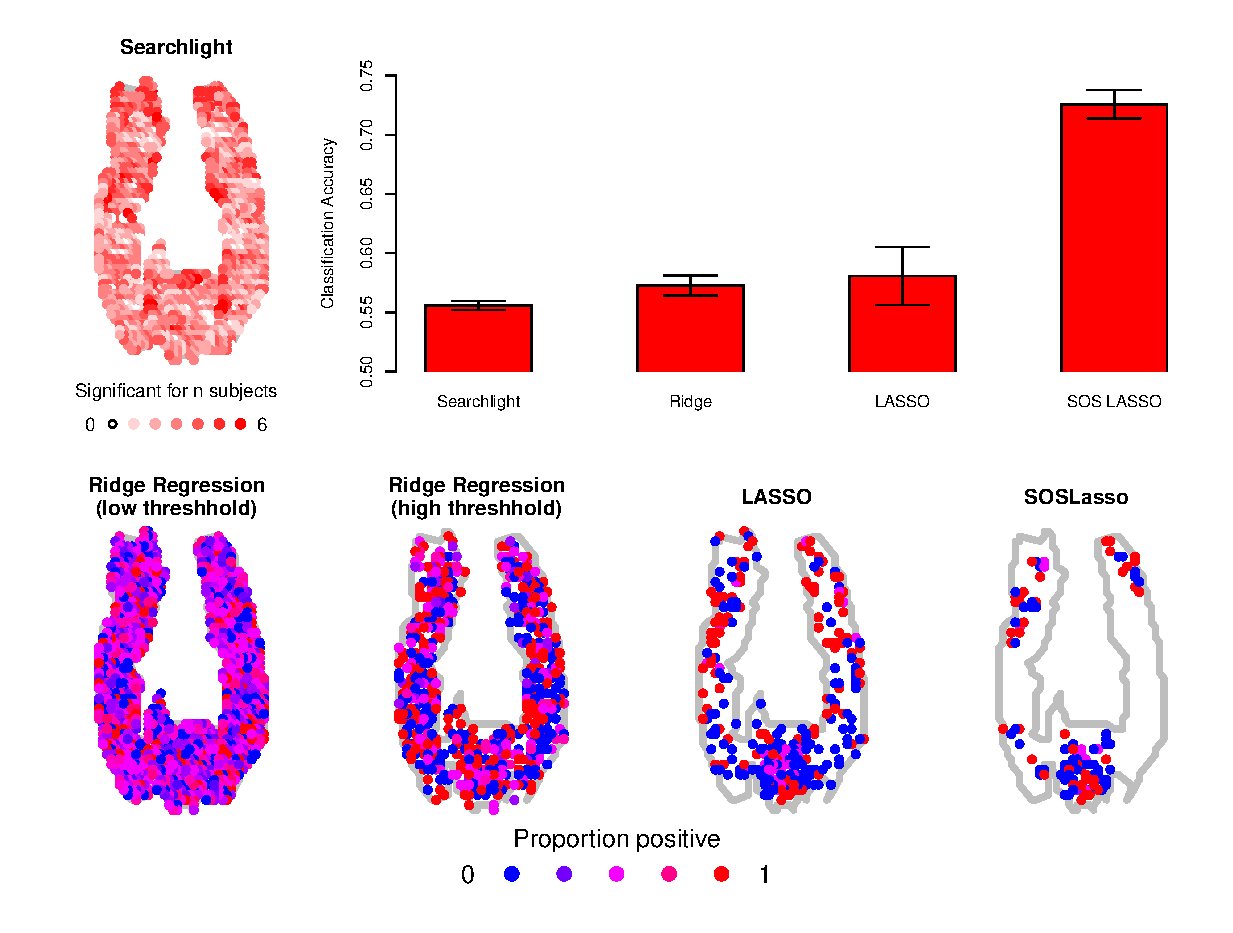
\includegraphics[width=.8\textwidth]{figures/figure10.eps}
\caption{Results from applying different multivariate methods to the star-plus fMRI dataset. (A) The information maps yielded by applying different multivariate methods to the same ``star-plus'' dataset. Because the solutions are very sparse for {\lasso} and {\soslasso}, all voxels selected for any subject are plotted. For ridge regression, the plot shows voxels selected across all subjects under a lax and an aggressive elimination policy. For LASSO, ridge, and {\soslasso}, the blueness or redness of the dots conveys the proportion of the time each unit was assigned a positive weight over subjects. (B) Mean and standard error of the classifier cross-validation accuracy for each method across subjects in the star-plus dataset.}
\label{fig.brain}  
\end{figure*}

All methods exhibited significant above-chance cross-validation accuracy, indicating that they all discover some reliable structure. Figure \ref{fig.brain} presents the mean cross-validation accuracy of each method along with aggregate images of the brain regions identified as encoding useful structure by the different methods within one representative slice of the brain.  Identified voxels are aggregated across the Z plane and projected on a single horizontal section taken through the middle of the temporal lobe, with anterior regions toward the top. 

For searchlight, voxel coloring indicates the proportion of participants for whom the surrounding searchlight led to reliable above-chance classification. Though the map is not statistically thresholded in the usual manner (owing to the previously-noted limitations of the dataset), the color intensity gives a sense of what such a map would look like. The signal appears to be highly distributed all throughout the measured regions, similar to the model results obtained when the searchlight was too large. There are no regions where signal is obviously absent. 

In the remaining panels, red indicates voxels where high BOLD was associated with picture processing, blue indicates voxels where high BOLD was associated with sentence processing, and purple indicates voxels with different interpretations across individuals. For {\lasso}, selected voxels are sparsely distributed throughout the measured regions, with no discernable spatial topography apart from a denser clustering of blue voxels toward the occipital cortex. Most points are either red or blue because there was relatively little overlap in the selected voxels across subjects. The ridge regression plots show results at two levels of weight thresholding (10\% and 90\%). Here the voxel hue indicates the proportion of positive weights across individuals, while the intensity indicates the mean absolute value of the voxel weight across individuals. In both cases, the results are a ``purple haze'': almost everything is selected in some participant, and there is little apparent coherence across participants in how a given voxel encodes information. Finally, the {\soslasso} plot identifies fewer voxels overall, but these tend to be loosely localized within three regions: the occipital cortex, and left and right anterior temporal cortices. Within these regions, the direction of the classifier weights appears largely intermixed, consistent with the PDP hypothesis that the nature of the neural code can be highly variable both within and across individuals.

From these images, it is clear that the different methods do indeed yield very different conclusions about how the relevant signal is encoded. Which view are we to believe? Cross-validation accuracy of the different classifiers might provide one clue: presumably solutions that have done a better job identifying important components of the representation should show better cross-validation performance. We therefore compared the mean cross-validation accuracy across the different methods. For searchlight, this was measured in each participant by taking the mean accuracy over all searchlights individually showing reliable above-chance classification. The other methods each directly yield a single measure of accuracy for each participant. Means and standard errors of these figures across participants are shown in the top right panel of Figure \ref{fig.brain}. {\soslasso} shows significantly better performance than the other three methods, suggesting that it has done a better job of picking out useful representational structure in each individual.

A second way of assessing the different solutions is to compare them to \emph{a priori} expectations. In this case, recall that the authors of the star-plus study originally identified 7 regions of interest where they expected functional activations to carry important information. Thus we can inquire how well the solution for each method aligns with these expectations, by computing what proportion of the identified voxels fall within these 7 ROIs. For {\soslasso}, 65\% of the identified voxels on average across subjects fell into the expert-defined ROIs---significantly more than all other methods (44\% for LASSO, 26\% for both variants of ridge regression, and 22\% for searchlight, $p < 0.03$ for within-subject contrast to {\soslasso} for all methods).

